% (c) 2012 Claudio Carboncini - claudio.carboncini@gmail.com
% (c) 2012-2014 Dimitrios Vrettos - d.vrettos@gmail.com

\chapter{Divisione tra due polinomi}

\section{Polinomi in una sola variabile}

Ricordiamo la divisione tra due numeri, per esempio~$147:4$. Si tratta di trovare un quoziente~$q$ e un resto~$r<4$, in modo 
che~$147=q\cdot 4+r$. Un algoritmo per trovare questi due numeri è il seguente:
\begin{center}
 % (c) 2012 Dimitrios Vrettos - d.vrettos@gmail.com
\begin{tikzpicture}[x=5mm,y=5mm, font=\small]
\begin{scope}[font=\ttfamily]
\matrix  (a) [matrix of nodes, anchor=south]{
1&4&7&4\\
1&2&{}&3&6\\
&2&7\\
&2&4\\
&&3\\};
\end{scope}

\draw(a-1-4.north west)--(a-2-4.south west);
\draw(a-2-4.north west)--(a-2-5.north east);
\draw(a-2-1.south west)--(a-2-3.south east);
\draw(a-4-2.south west)--(a-4-3.south east);

\node (d) at (-6,6) {dividendo};
\node (r) at (-6,0) {resto};
\node (di) at (6,6) {divisore};
\node (q) at (6,3) {quoziente};

\begin{scope}[->]
\draw (d.east)--(a-1-1.west);
\draw (r.east)--(a-5-3.west);
\draw (di.west)--(a-1-4.east);
\draw (q.west)--(a-2-5.east);
\end{scope}
\end{tikzpicture}
\end{center}
Verifichiamo che~$147=36\cdot 4+3$, dunque~$q=36$ e~$r=3$ soddisfano la nostra richiesta.

In questo paragrafo ci proponiamo di estendere questo algoritmo dal calcolo numerico al calcolo letterale, in particolare alla divisione tra polinomi.

Nell'insieme dei polinomi in una sola variabile, ad esempio~$x$, vogliamo definire l'operazione di divisione, cioè, assegnati
due polinomi, $A(x)$ \emph{dividendo} e~$B(x)$ \emph{divisore}, vogliamo determinare altri due polinomi, $Q(x)$ \emph{quoziente} e~$R(x)$ \emph{resto},
con grado di~$R(x)$ minore del grado di~$B(x)$, per i quali:~$A(x) = B(x){\cdot}Q(x) + R(x)$.

Per eseguire l'operazione si usa un algoritmo molto simile a quello usato per la divisione tra numeri interi. Illustriamolo con un esempio.

\begin{exrig}
 \begin{esempio}
Eseguire la divisione tra i polinomi~$A(x)=3x^{4}+5x-4x^{3}-1$ e~$B(x)=3x^{2}-1$.

Prima di eseguire l'algoritmo dobbiamo sempre controllare che:
\begin{itemize*}
 \item il dividendo sia di grado maggiore o uguale a quello del divisore:~$A(x)$ ha grado~$4$ e $B(x)$ ha grado~$2$;
 \item i polinomi siano ordinati secondo le potenze decrescenti della variabile, in questo caso la~$x$; poiché ciò
    non è vero, riscriviamo~$A(x)$ ordinato:~$A(x)=3x^{4}-4x^{3}+5x-1$;
 \item dividendo e divisore siano in forma completa, cioè abbiano i termini con tutti i gradi; nel nostro esempio, i due polinomi non sono in
    forma completa, quindi inseriamo i termini mancanti ponendo~0 come coefficiente delle potenze mancanti:
    \[A(x)=3x^{4}-4x^{3}+0x^{2}+5x-1;\quad B(x)=3x^{2}+0x-1.\]
\end{itemize*}
\paragraph{Passo I}
 Disponiamo i polinomi secondo il seguente schema, del tutto simile a quello usato per la divisione tra numeri.
\begin{center}
 % (c) 2012 Dimitrios Vrettos - d.vrettos@gmail.com
\begin{tikzpicture}[font=\small]

\matrix  (a) [matrix of  nodes, anchor=south,text depth=1mm]{
$3x^4$&$-4x^3$&$+0x^2$&$+5x$&$-1$ &$3x^2$&$+0x$&$-1$\\};

\draw(a-1-6.north west)--(a-1-6.south west);
\draw(a-1-6.south west)--(a-1-8.south east);

\begin{scope}[font=\scriptsize]
 \node[above] (d) at (a-1-3.north) {dividendo};
 \node[below] (r) at (a-1-3.south) {Spazio per i calcoli};
 \node [above](di) at (a-1-7.north) {divisore};
 \node [below] (q) at (a-1-7.south) {Spazio per il quoziente};
\end{scope}
\end{tikzpicture}
\end{center}
\paragraph{Passo II}
 Dividiamo il primo termine del dividendo per il primo termine del divisore, otteniamo~$x^{2}$ che è il primo termine del quoziente;
 esso va riportato nello spazio dedicato al quoziente.
\begin{center}
 % (c) 2012 Dimitrios Vrettos - d.vrettos@gmail.com
\begin{tikzpicture}[font=\small]
 \pgfsetmatrixrowsep{5mm}

\matrix  (a) [matrix of  nodes, anchor=south, minimum width=9mm, ,nodes={text depth=1mm}]{
$3x^4$&$-4x^3$&$+0x^2$&$+5x$&$-1$ &$3x^2$&$+0x$&$-1$\\
&&&&&$x^2$\\};

 \draw(a-1-6.north west)--(a-2-6.south west);
 \draw(a-1-6.south west)--(a-1-8.south east);

 \begin{scope}[->,red]
\draw (a-1-1.north) .. controls +(up:1cm) and +(up:1.5cm).. node[above] {$:$} (a-1-6);
\draw (a-1-6.south) -- (a-2-6.north);
 \end{scope}

\end{tikzpicture}
\end{center}
\paragraph{Passo III}
 Moltiplichiamo il primo termine ottenuto per tutti i termini del divisore e trascriviamo il risultato del prodotto sotto il dividendo,
avendo cura, per essere facilitati nel calcolo, di:
\begin{itemize*}
\item incolonnare i termini con lo stesso grado, ossia scrivere i risultati del prodotto in ordine da sinistra verso destra;
\item cambiare tutti i segni ottenuti, in questo modo risulta più pratico eseguire la somma algebrica dei polinomi invece della sottrazione.
\end{itemize*}
\begin{center}
 % (c) 2012 Dimitrios Vrettos - d.vrettos@gmail.com
\begin{tikzpicture}[font=\small]
\pgfsetmatrixrowsep{2mm}

\matrix  (a) [matrix of  nodes, anchor=south, minimum width=9mm, text depth=1mm]{
$3x^4$&$-4x^3$&$+0x^2$&$+5x$&$-1$ &$3x^2$&$+0x$&$-1$\\
$-3x^4$&$-0x^3$&$+x^2$&&&$x^2$\\};

 \draw(a-1-6.north west)--(a-2-6.south west);
\draw(a-1-6.south west)--(a-1-8.south east);

\begin{scope}[->,red, dashed]
 \draw (a-1-7.south) -- (a-2-6.east);
  \draw (a-2-6.west) -- (a-2-3.east);
 \end{scope}

\end{tikzpicture}

\end{center}
\paragraph{Passo IV}
 Sommiamo il dividendo con il polinomio sottostante e riportiamo il risultato in un'altra riga. Questo polinomio si chiama primo resto parziale.
 Notiamo che ha grado~$3$, maggiore del grado~$2$ del divisore, pertanto la divisione va continuata.

\begin{center}
 % (c) 2012 Dimitrios Vrettos - d.vrettos@gmail.com
\begin{tikzpicture}[font=\small]

\matrix  (a) [matrix of  nodes, anchor=south, minimum width=9mm, text depth=1mm]{
$3x^4$&$-4x^3$&$+0x^2$&$+5x$&$-1$ &$3x^2$&$+0x$&$-1$\\
$-3x^4$&$-0x^3$&$+x^2$&&{}&$x^2$\\
{}&$-4x^3$&$+x^2$&$+5x$&$-1$\\};

 \draw(a-1-6.north west)--(a-2-6.south west);
\draw(a-1-6.south west)--(a-1-8.south east);
\draw (a-2-1.south west) -- (a-2-5.south east);

\end{tikzpicture}
\end{center}
\paragraph{Passo V}
 Ripetiamo il procedimento tra il resto parziale ottenuto, $-4x^{3}+x^{2}+5x-1$ e il divisore~$3x^{2}+0x-1$. Dividiamo il primo termine del resto che
 è~$-4x^{3}$ per il primo termine del divisore che è~$3x^{2}$. Otteniamo~$-{\frac{4}{3}}x$ che è il secondo termine del quoziente.
% \newpage
\begin{center}
 \input{./lbr/chap12/fig006_div.pgf}
\end{center}
\paragraph{Passo VI}
 Proseguiamo moltiplicando~$-{\frac{4}{3}}x$ per~$B(x)$, riportiamo il risultato del prodotto, con segno opposto, sotto i
 termini del primo resto parziale e addizioniamo i due polinomi.
\begin{center}
 % (c) 2012 Dimitrios Vrettos - d.vrettos@gmail.com
\begin{tikzpicture}[font=\small]

\matrix  (a) [matrix of  nodes, anchor=south, minimum width=9mm, ,nodes={text depth=2.5mm}]{
$3x^4$&$-4x^3$&$+0x^2$&$+5x$&$-1$ &$3x^2$&$+0x$&$-1$\\
$-3x^4$&$-0x^3$&$+x^2$&&{}&$x^2$&$-\displaystyle\frac{4}{3}x$\\
{}&$-4x^3$&$+x^2$&$+5x$&$-1$\\
{}&$-4x^3$&$+0x^2$&$-\displaystyle\frac{4}{3}x$&{}\\
{}&&$x^2$&$+\displaystyle\frac{11}{3}x$&$-1$\\};

 \draw(a-1-6.north west)--(a-2-6.south west);
 \draw(a-1-6.south west)--(a-1-8.south east);
 \draw (a-2-1.south west) -- (a-2-5.south east);
\draw (a-4-2.south west) -- (a-4-5.south east);
\end{tikzpicture}
\end{center}
\paragraph{Passo VII}
 Possiamo ripetere per l'ultima volta il procedimento precedente tra il resto parziale~$R_{p}(x)=x^{2}+\frac{11}{3}x-1$ e
 il divisore~$B(x)$ in quanto hanno lo stesso grado. Dividendo il termine di grado maggiore di~$R_{p}(x)$, che è~$x^{2}$,
 per il termine di grado maggiore di~$B(x)$ che è~$3x^{2}$ si ottiene~$\frac{1}{3}$ che è il terzo termine del polinomio quoziente.
\begin{center}
 \input{./lbr/chap12/fig008_div.pgf}
\end{center}

Non possiamo più ripetere l'algoritmo poiché il resto ottenuto ha grado minore del grado del divisore.

In conclusione~$A(x):B(x)$ ha quoziente~$Q(x)=x^{2}-\dfrac{4}{3}x+\dfrac{1}{3}$ e resto~$R(x)={\dfrac{11}{3}}x-\dfrac{2}{3}$.

\paragraph{Verifica}
Verifichiamo se abbiamo svolto correttamente i calcoli; dovrebbe risultare, come detto sopra:$\quad A(x)=Q(x)\cdot B(x)+R(x)$.
\begin{equation*}
\begin{split}
\left(3x^{2}-1\right)\left(x^{2}-\frac{4}{3}x+\frac{1}{3}\right)+\frac{11}{3}x &= 3x^{4}-4x^{3}-x^{2}+\frac{4}{3}x-\frac{1}{3}+\frac{11}{3}x-\frac{2}{3}\\
                                        &= 3x^{4}-4x^{3}+\frac{15}{3}x-\frac{3}{3}\\
                                        &=x^{4}-4x^{3}+5x-1\\
                                        &=A(x).
\end{split}
\end{equation*}
I polinomi~$Q(x)$ e~$R(x)$ soddisfano quindi le nostre richieste. Ma sono unici? È sempre possibile trovarli? A queste domande risponde il seguente teorema.
 \end{esempio}
\end{exrig}

\begin{teorema}[Divisione euclidea]
 Siano~$A(x)$ e~$B(x)$ due polinomi in una sola variabile, esistono e sono unici due polinomi~$Q(x)$ e~$R(x)$, con grado di~$R(x)$
 minore o uguale del grado di~$B(x)$, tali che~$A(x)=Q(x)\cdot B(x)+R(x)$.
\end{teorema}

\osservazione Nel caso in cui il grado di~$A(x)$ sia minore del grado di~$B(x)$ il teorema resta valido, in questo caso~$Q(x)=0$ e~$R(x)=A(x)$.
Nel caso di polinomi in più variabili il teorema della divisione euclidea non vale.

\begin{definizione}
 Si dice che un polinomio~$A$ (dividendo) è \emph{divisibile} per un polinomio~$B$ (divisore)
 se esiste un polinomio~$Q$ (quoziente) per il quale~$A=Q\cdot B$.
\end{definizione}

\begin{exrig}
 \begin{esempio}
 Eseguiamo la divisione tra~$A(x)=x^{3}-2x^{2}+x-2$ e~$B(x)=x^{2}+1$.
I due polinomi sono ordinati secondo potenze decrescenti della variabile, il grado di~$A$ è maggiore del grado di~$B$ e quest'ultimo
deve essere completo. Inseriamoli nello schema per eseguire l'algoritmo. Risulta:
$\left(x^{3}-2x^{2}+x-2\right):\left(x^{2}+1\right)=(x-2)$; il resto~$R(x)$ è il polinomio nullo e~$A(x)$ è divisibile per~$B(x)$.
Infatti~$\left(x^{2}+1\right)\cdot (x-2)=\left(x^{3}-2x^{2}+x-2\right)$.
\begin{center}
 % (c) 2012 Dimitrios Vrettos - d.vrettos@gmail.com
\begin{tikzpicture}[font=\small]

\matrix  (a) [matrix of  nodes, anchor=south, minimum width=9mm,nodes={text depth=1mm}]{
$x^3$&$-2x^2$&$+x$&$-2$ &$x^2$&$+0x$&$+1$\\
$-x^3$&$-0x^2$&$-x$&{}&$x$&$-2$\\
{}&$-2x^2$&$+0x$&$-2$\\
{}&$-2x^2$&$+0x$&$-2$\\
&&&$0$&{}\\
};

\draw(a-1-5.north west)--(a-2-5.south west);
\draw(a-1-5.south west)--(a-1-7.south east);
 \draw (a-2-1.south west) -- (a-2-4.south east);
 \draw (a-4-2.south west) -- (a-4-4.south east);
\end{tikzpicture}\vspace*{-1.10ex}
\end{center}
 \end{esempio}
\end{exrig}

In conclusione, se~$A(x)$ è un polinomio di grado~$n$ e~$B(x)$ un polinomio di grado~$m$ con~$n\ge m$, quando si esegue
la divisione tra~$A$ e~$B$ si ottiene un polinomio quoziente~$Q(x)$ di grado~$n-m$ e un polinomio~$R(x)$ di grado~$g<m$.
Si dimostra che i polinomi~$Q(x)$ e~$R(x)$ sono unici.

Se~$R(x)$ è il polinomio nullo, la divisione è esatta e il polinomio~$A$ è divisibile per il polinomio~$B$.
Se~$n<m$, allora la divisione non si può eseguire e si ottiene la frazione algebrica~$\frac{A}{B}$.

\vspazio\ovalbox{\risolvii \ref{ese:12.1}, \ref{ese:12.2}, \ref{ese:12.3}, \ref{ese:12.4}, \ref{ese:12.5}}

\section{Polinomi in più variabili}
Per la divisione tra polinomi in più variabili riportiamo soltanto qualche esempio.
\begin{exrig}
 \begin{esempio}
Siano~$A(a\text{,~}b)=3a^{2}b+4ab^{2}+3a^{3}-2b^{3}$ e~$B(a\text{,~}b)=a-3b$ rispettivamente dividendo e divisore di una divisione tra polinomi;
essi sono due polinomi omogenei nelle due variabili~$a$ e~$b$ rispettivamente di grado~$3$ e grado~$1$.

Per eseguire la divisione procediamo come nel caso di polinomi in una sola variabile.
Dividiamo il polinomio~$A(a\text{,~}b)=3a^{2}b+4ab^{2}+3a^{3}-2b^{3}$ per il polinomio~$B(a\text{,~}b)=a-3b$ rispetto alla variabile~$a$.
Controlliamo le condizioni:
\begin{itemize*}
\item $A$ e~$B$ sono ordinati rispetto alla variabile $a$? No, $A$ non lo è. Quindi ordiniamo~$A$:
\[A(a\text{,~}b)=3a^{3}+3a^{2}b+4ab^{2}-2b^{3};\]
\item il grado di~$A$ è maggiore o uguale al grado di~$B$? Sì;
\item $A$ e~$B$ sono completi rispetto alla variabile~$a$? Sì.
\end{itemize*}
Costruiamo lo schema per eseguire l'algoritmo e procediamo:
\begin{center}
 % (c) 2012 Dimitrios Vrettos - d.vrettos@gmail.com
\begin{tikzpicture}[x=6mm,  y=6mm]
  \newcounter{num}
  \setcounter{num}{0}
  
  \draw[color=gray, step=6mm] (0,0) grid (8,10);
  \foreach \y in {9,8,...,0}{
    \foreach \x in {0,1,...,7}{
      \stepcounter{num}
      \ifnum \thenum<28
	\draw[xshift=3mm,yshift=3mm] (\x , \y ) node {\thenum};
      \fi
    }
  }
  
  \foreach \j in {10,9,8,...,0}
    \foreach \i in {0,1,...,8}
      \draw[] (\i , \j ) node[fill=white] {};
\end{tikzpicture}
\end{center}
Il quoziente è~$Q =\ldots \ldots \ldots$; il resto~$R = 118b^{3}$

Verifica~$\ldots \ldots \ldots \ldots \ldots \ldots$

Se avessimo eseguito la divisione rispetto alla variabile~$b$, avremmo ottenuto stesso quoziente e stesso resto? Proviamo.
Controlliamo le condizioni:
\begin{itemize*}
\item $A$ e~$B$ sono ordinati rispetto alla variabile~$b$? No. Ordinando~$A$, risulta:
\[A(a\text{,~}b)=-2b^{3}+4ab^{2}+3a^{2}b+3a^{3}+3a^{2}b;\]
e ordinando~$B$, risulta
\[B(a\text{,~}b)=-3b+a;\]
\item il grado di~$A$ è maggiore o uguale al grado di~$B$? Sì;
\item $A$ e~$B$ sono completi rispetto alla variabile~$b$? Sì.
\end{itemize*}
Costruisci lo schema dell'algoritmo e concludi.
 \end{esempio}
\end{exrig}
\ovalbox{\risolvii \ref{ese:12.6}, \ref{ese:12.7}}

\section{Regola di Ruffini}\label{sect:regola_di_Ruffini}

Per eseguire la divisione tra due polinomi in una sola variabile, \emph{nel caso in cui il
divisore sia di grado~1} si può applicare una regola nota come \emph{regola
di Ruffini}\footnote{dal nome del matematico e medico italiano Paolo Ruffini (1765 - 1822).} (o \emph{divisione sintetica}) e che si basa sui seguenti teoremi.

\begin{teorema}
 Il resto della divisione di un polinomio~$A(x)$ per un
binomio del tipo~$(x-k)$ è uguale al valore che~$A(x)$ assume quando
al posto della variabile $x$ si sostituisce il valore $k$, $R=A(k)$.
\end{teorema}

\begin{proof}
 Dalla divisione di~$A(x)$ per~$x-k$ otteniamo la seguente
uguaglianza:
\[A(x)=(x-k)\cdot Q(x)+R\]
in cui si è scritto~$R$ anziché $R(x)$, poiché è
una costante.

Essendo tale relazione valida per qualsiasi valore che si attribuisce
alla variabile~$x$, sostituiamo al suo posto il valore
$k$ e otteniamo:

\[A(k)=\underbrace{(k-k)}_{0}\cdot Q(k)+R=R.\]

Ciò vuol dire che il valore assunto da~$A(x)$
quando~$x=k$ è proprio uguale al resto della divisione.
\end{proof}

\begin{teorema}[di Ruffini]
 Condizione necessaria e sufficiente affinché un
polinomio~$A(x)$ sia divisibile per un binomio del tipo~$(x-k)$ è
che risulti~$A(k)=0$.
\end{teorema}

\begin{proof}
\emph{Prima implicazione}:~$A(x)$ divisibile per~$(x-k)\:\Rightarrow\: A(k)=0$.

Poiché $A(x)$ è divisibile per~$(x-k)$, per definizione di divisibilità deve essere~$R=0$. Ma, per il
teorema del resto, $A(k)=R=0$, quindi, per la proprietà transitiva
dell'uguaglianza, $A(k)=0$.

\emph{Seconda implicazione}:~$A(k)=0\:\Rightarrow\: A(x)$
divisibile per~$(x-k)$.

Il resto della divisione del polinomio~$A(x)$ per il binomio~$x-k$,
per il teorema del resto risulta~$R=A(k)$ e per ipotesi~$A(k)=0$,
ne segue che~$R=0$. Per definizione di divisibilità, essendo il
resto della divisione zero, segue che~$A(x)$ è divisibile per~$(x-k)$.
\end{proof}


\begin{procedura}
 Dividere un polinomio con la regola di Ruffini:

 \begin{enumeratea}
 \item calcolo del resto;
\item applicazione del procedimento di divisione;
\item verifica.
 \end{enumeratea}
\end{procedura}


\begin{exrig}
 \begin{esempio}
$\left(a^{2}-3a+1\right):(a-1).$

Dividiamo con la regola di Ruffini il polinomio~$A(a)=a^{2}-3a+1$ per
il binomio~$B(a)=a-1$; cerchiamo quoziente~$Q(a)$ e resto~$R(a)$.

\paragraph{Passo I} \emph{Calcolo del polinomio resto.}

Si considera il termine numerico del polinomio divisore cambiato di
segno (nell'esempio è~1) e si sostituisce alla
lettera del polinomio dividendo~$A(1)$:~$1^{2}-3\cdot 1 + 1 = 1 - 3 + 1 = -1$.

Il resto della divisione è~$-1$.

\paragraph{Passo II} \emph{Applicazione del procedimento di divisione.}

Disegnare il seguente schema di Ruffini: scrivere i coefficienti
numerici del polinomio dividendo, secondo le potenze decrescenti della
variabile. Se manca un termine occorre mettere~0.
L'ultimo termine numerico è messo esternamente alla
griglia. Nell'angolo a sinistra dello schema si pone il
termine numerico del polinomio divisore cambiato di segno,
nell'esempio è~1.

\begin{center}
% (c) 2012 Dimitrios Vrettos - d.vrettos@gmail.com
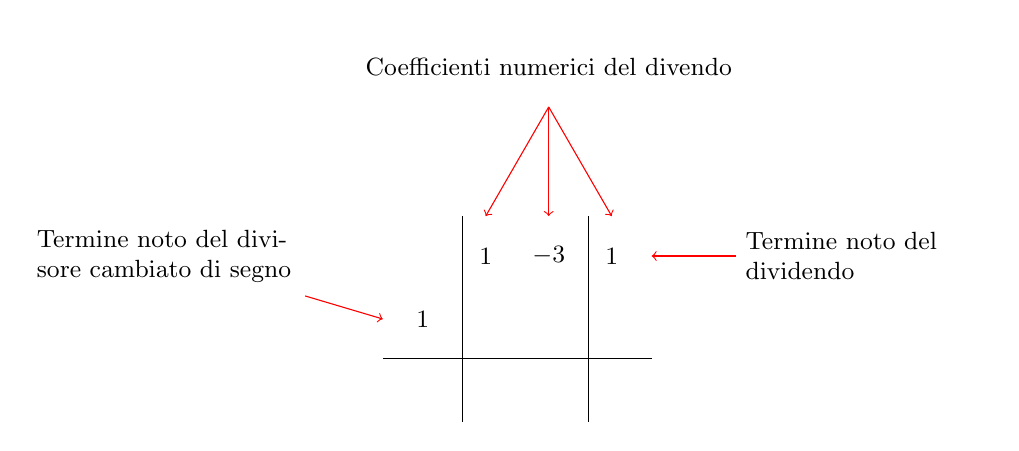
\begin{tikzpicture}[font=\small,x=8mm, y=8mm, minimum size=10mm]

\node (a0) at (0,0) {};
\node (a1) at (1,0) {1};
\node (a2) at (2,0) {$-3$};
\node (a3) at (3,0) {1};

\node(a4) at (0,-1) {1};
\node (a5) at (1,-1) {};
\node (a6) at (2,-1) {};
\node (a7) at (3,-1) {};

\node (a8) at (0,-2) {};
\node (a9) at (1,-2) {};
\node (a10) at (2,-2) {};
\node (a11) at (3,-2) {};

\draw (a0.north east)--(a8.south east);
 \draw (a4.south west)--(a7.south east);
\draw (a2.north east)--(a10.south east);

\node (b) at (2,3) {Coefficienti numerici del divendo};
\node[text width=3.4cm] (c) at (-4,0){Termine noto del divisore cambiato di segno};
\node[text width=3cm] (d) at (7,0) {Termine noto del dividendo};

\begin{scope}[->, red]
\foreach \x in {a1.north, a2.north, a3.north}
	\draw (b.south)--(\x);
\draw (c) -- (a4.west);
\draw (d)-- (a3.east);
\end{scope}

\end{tikzpicture}
\end{center}

\begin{multicols}{2}
 Il primo termine si riporta inalterato nella parte sottostante:
\begin{center}
\input{./lbr/chap12/fig013_ruf.pgf}
\end{center}
\end{multicols}

\begin{multicols}{2}
 Moltiplicare il termine noto del divisore (cambiato di segno) per il
primo coefficiente appena trascritto e riportare il risultato sotto il
secondo coefficiente
\begin{center}
\input{./lbr/chap12/fig014_ruf.pgf}
\end{center}
\end{multicols}

\begin{multicols}{2}
 Sommare i due termini appena incolonnati~$-3+1=-2$.
\begin{center}
\input{./lbr/chap12/fig015_ruf.pgf}
\end{center}
\end{multicols}

\begin{multicols}{2}
 Moltiplicare il termine noto del divisore (cambiato di segno) per la
somma appena ottenuta~$1\cdot (-2)=-2$.
\begin{center}
% (c) 2012 Dimitrios Vrettos - d.vrettos@gmail.com
\begin{tikzpicture}[font=\small,x=8mm, y=8mm, minimum size=10mm]

\node (a0) at (0,0) {};
\node (a1) at (1,0) {1};
\node (a2) at (2,0) {$-3$};
\node (a3) at (3,0) {1};

\node(a4) at (0,-1) {1};
\node (a5) at (1,-1) {};
\node (a6) at (2,-1) {1};
\node (a7) at (3,-1) {$-2$};

\node (a8) at (0,-2) {};
\node (a9) at (1,-2) {1};
\node (a10) at (2,-2) {$-2$};
\node (a11) at (3,-2) {};

\draw (a0.north east)--(a8.south east);
 \draw (a4.south west)--(a7.south east);
\draw (a2.north east)--(a10.south east);

\begin{scope}[->,red]
\draw (a4.east)--(a10.west);
\draw (a10.east)--(a7.south);
\end{scope}
\end{tikzpicture}

\end{center}
\end{multicols}
%\newpage
\begin{multicols}{2}
 Addizionare gli ultimi due numeri incolonnati~$1-2=-1$.
\begin{center}
% (c) 2012 Dimitrios Vrettos - d.vrettos@gmail.com
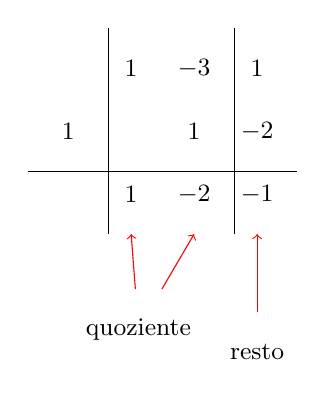
\begin{tikzpicture}[font=\small,x=8mm, y=8mm, minimum size=10mm]

\node (a0) at (0,0) {};
\node (a1) at (1,0) {1};
\node (a2) at (2,0) {$-3$};
\node (a3) at (3,0) {1};

\node(a4) at (0,-1) {1};
\node (a5) at (1,-1) {};
\node (a6) at (2,-1) {1};
\node (a7) at (3,-1) {$-2$};

\node (a8) at (0,-2) {};
\node (a9) at (1,-2) {1};
\node (a10) at (2,-2) {$-2$};
\node (a11) at (3,-2) {$-1$};

\draw (a0.north east)--(a8.south east);
 \draw (a4.south west)--(a7.south east);
\draw (a2.north east)--(a10.south east);

\node[below left of=a10,below=5mm](q)  {quoziente};
\node[below of=a11, below=5mm](r)  {resto};
\begin{scope}[->,red]
\draw (q)--(a9.south);
\draw (q)--(a10.south);
\draw (r)--(a11.south);
\end{scope}
\end{tikzpicture}
\end{center}
\end{multicols}

Infine si ricostruisce il polinomio quoziente, tenendo presente che i
coefficienti numerici sono quelli trovati da questa divisione, cioè~1
e~$-2$. Quoziente e resto sono allora~$Q(x)=a-2$ e~$R=-1$.

\paragraph{Passo III}\emph{Verifica}

Come nella divisione con i numeri, si moltiplica il polinomio risultato
per il polinomio divisore e si somma il polinomio resto. Il risultato
deve essere il polinomio dividendo.
\[(a - 2)(a - 1) + (-1) = a^{2} - a - 2a + 2 - 1 =a^{2}-3a + 1.\]
 \end{esempio}

\begin{esempio}
$(4x^{3} - 5x + 6): (x + 1).$

Applicazione del procedimento di divisione
\begin{center}
% (c) 2012 Dimitrios Vrettos - d.vrettos@gmail.com
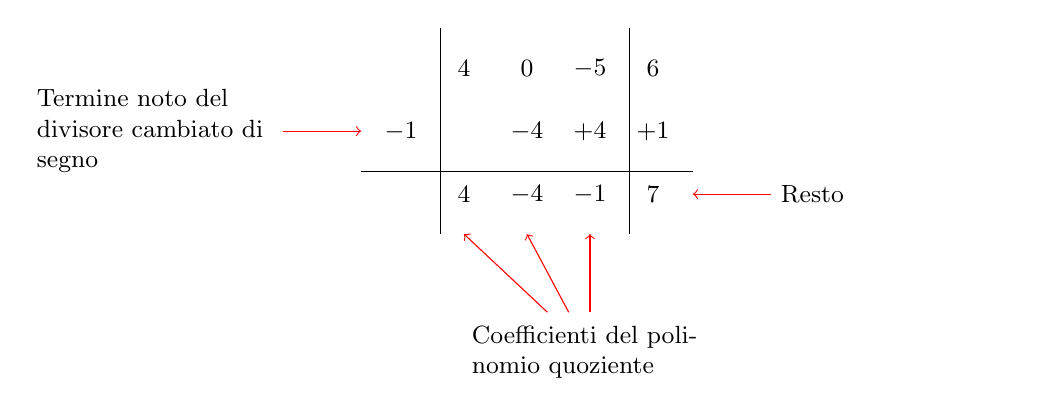
\begin{tikzpicture}[font=\small,x=8mm, y=8mm, minimum size=10mm]

\node (a0) at (0,0) {};
\node (a1) at (1,0) {4};
\node (a2) at (2,0) {0};
\node (a3) at (3,0) {$-5$};
\node (a4) at (4,0) {6};

\node(a5) at (0,-1) {$-1$};
\node (a6) at (1,-1) {};
\node (a7) at (2,-1) {$-4$};
\node (a8) at (3,-1) {$+4$};
\node (a9) at (4,-1) {$+1$};

\node (a10) at (0,-2) {};
\node (a11) at (1,-2) {4};
\node (a12) at (2,-2) {$-4$};
\node (a13) at (3,-2) {$-1$};
\node (a14) at (4,-2) {7};

\draw (a0.north east)--(a10.south east);
 \draw (a5.south west)--(a9.south east);
\draw (a3.north east)--(a13.south east);

 \node[text width=3cm, left of=a5, left=5mm](b)  {Termine noto del divisore cambiato di segno};
 \node[text width=3cm, below of=a13, below=5mm](c)  {Coefficienti del polinomio quoziente};
 \node[text width=3cm, right of=a14, right=5mm](d)  {Resto};
 \begin{scope}[->,red]
 \draw (b)--(a5.west);
 \draw (d)--(a14);
\foreach \x in {a11,a12,a13}
\draw (c)--(\x.south);
 \end{scope}
\end{tikzpicture}
\end{center}
\[Q(x)=4x^{2}-4x-1 \qquad R=7.\]
\end{esempio}

\textit{Verifica.}

\[Q(x)\cdot B(x)+R=A(x)\]

\[\left(4x^{2}-4x-1\right)\cdot (x+1)+7=4x^{3}+4x^{2}-4x-x-1+7=4x^{3}-5x+6\]

Vediamo il caso in cui il binomio che fa da divisore ha coefficiente
numerico della variabile diverso da~1.


\begin{esempio}
 Dividere con la regola di Ruffini~$\left(2x^{4}-x^{3}-4x^{2}+2x+7\right):(2x-1)$.

In questo tipo di esercizi si deve rendere il divisore del tipo~$x+n$,
quindi nel nostro caso si deve dividere sia il dividendo sia il
divisore per~2; sappiamo, infatti, dalla proprietà invariantiva della
divisione che dividendo per uno stesso numero dividendo e divisore il
quoziente della divisione non cambia. Il resto invece risulterà
diviso per~2. Quindi applichiamo l'algoritmo precedente
e \emph{ricordiamoci al termine della divisione di moltiplicare il
resto per}~2.

La divisione allora diventa
$\left(x^{4}-\frac{1}{2}x^{3}-2x^{2}+x+\frac{7}{2}\right):\left(x-\frac{1}{2}\right)$.
\end{esempio}
\end{exrig}

\ovalbox{\risolvii \ref{ese:12.8}, \ref{ese:12.9}, \ref{ese:12.10}, \ref{ese:12.11}, \ref{ese:12.12}}

\subsection{Calcolo del resto}

Si considera il termine numerico del polinomio divisore cambiato di
segno (nell'esempio precedente è~$+{\frac{1}{2}}$) e si
sostituisce alla lettera che compare nel polinomio dividendo. Il risultato che si
ottiene è il resto della
divisione~$\left(\frac{1}{2}\right)^{4}-\frac{1}{2}\left(\frac{1}{2}\right)^{3}-2\left(\frac{1}{2}\right)^{2}+\frac{1}{2}+\frac{7}{2}=-\frac{1}{16}-\frac{1}{2}+\frac{1}{2}+\frac{7}{2}=\frac{7}{2}$.

Applicazione del procedimento di divisione.
\begin{center}
 % (c) 2012 Dimitrios Vrettos - d.vrettos@gmail.com
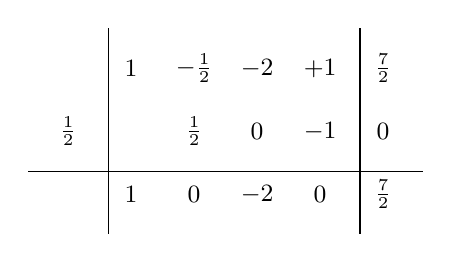
\begin{tikzpicture}[font=\small,x=8mm, y=8mm, minimum size=10mm]

\node (a0) at (0,0) {};
\node (a1) at (1,0) {1};
\node (a2) at (2,0) {$-\frac{1}{2}$};
\node (a3) at (3,0) {$-2$};
\node (a4) at (4,0) {$+1$};
\node (a5) at (5,0) {$\frac{7}{2}$};

\node(a6) at (0,-1) {$\frac{1}{2}$};
\node (a7) at (1,-1) {};
\node (a8) at (2,-1) {$\frac{1}{2}$};
\node (a9) at (3,-1) {0};
\node (a10) at (4,-1) {$-1$};
\node (a11) at (5,-1) {0};

\node (a12) at (0,-2) {};
\node (a13) at (1,-2) {1};
\node (a14) at (2,-2) {0};
\node (a15) at (3,-2) {$-2$};
\node (a16) at (4,-2) {0};
\node (a17) at (5,-2) {$\frac{7}{2}$};

\draw (a0.north east)--(a12.south east);
 \draw (a6.south west)--(a11.south east);
\draw (a4.north east)--(a16.south east);

\end{tikzpicture}
\end{center}

Adesso si pone la lettera per ogni termine del polinomio risultato
partendo dal grado del polinomio dividendo diminuito di~1. Il risultato
è quindi il polinomio~$x^{3}-2x$, il resto è~$\frac{7}{2}\cdot2=7$.

\paragraph{Verifica}
Per la proprietà della divisione si moltiplica il quoziente per il
polinomio divisore e si somma il resto ottenuto. Il risultato deve
essere il polinomio dividendo.

\[\left(x^{3}-2x\right)(2x-1)+7=2x^{4}-x^{3}-4x^{2}+2x+7.\]

In generale, se si vuole dividere il polinomio~$A(x)$ per il binomio~$(nx-\alpha)$, utilizzando la proprietà invariantiva della
divisione, si divide dividendo e divisore per~$n$, così da ottenere un divisore con coefficiente 1 per il termine di primo grado. Quindi si può effettuare la divisione ottenendo il quoziente $Q(x)$ ed il resto $R$. Per ottenere il resto della divisione di
partenza occorre moltiplicare $R$ per il coefficiente~$n$.
Infatti si ha:~$A(x)=(nx-\alpha)Q(x)+R $
e, dividendo ambo i membri per~$n$, si ha:
\[\frac{A(x)}{n}=\left(x-\frac{\alpha }{n}\right)Q(x)+\frac{R}{n}.\]
\ovalbox{\risolvii \ref{ese:12.13}, \ref{ese:12.14}, \ref{ese:12.15}, \ref{ese:12.16}, \ref{ese:12.17}, \ref{ese:12.18}}
\newpage
% (c) 2012 Claudio Carboncini - claudio.carboncini@gmail.com
% (c) 2012 -2014 Dimitrios Vrettos - d.vrettos@gmail.com

\section{Esercizi}
\subsection{Esercizi dei singoli paragrafi}
\subsubsection*{\thechapter.1 - Divisioni in una variabile}

\begin{esercizio}
\label{ese:12.1}
Completa la divisione
\begin{center}
 % (c) 2012 Dimitrios Vrettos - d.vrettos@gmail.com
\begin{tikzpicture}[font=\small]

\matrix  (a) [matrix of  nodes, anchor=south, minimum width=9mm, ,nodes={text depth=2.5mm}]{
$7x^4$&$+0x^3$&$-5x^2$&$+x$&$-1$ &$2x^2$&$+0x$&$-1$\\
{}&{}&$\ldots$&{}&{}&$\displaystyle\frac{7}{2}x$&\ldots\\
{}&{}&$-\displaystyle\frac{3}{2}x^2$&$+x$&$-1$\\
{}&{}&{}&\ldots&{}\\
&&&$x$&$-\displaystyle\frac{7}{4}$\\
};

\draw(a-1-6.north west)--(a-2-6.south west);
\draw(a-1-6.south west)--(a-1-8.south east);
 \draw (a-2-1.south west) -- (a-2-5.south east);
 \draw (a-4-2.south west) -- (a-4-5.south east);
\end{tikzpicture}
\end{center}
\end{esercizio}

\begin{esercizio}[\Ast]
\label{ese:12.2}
Esegui le divisioni tra polinomi.
 \begin{enumeratea}
 \item $\left(3x^{2}-5x+4\right):\left(2x-2\right)$;
 \item $\left(4x^{3}-2x^{2}+2x-4\right):\left(3x-1\right)$;
 \item $\left(5a^{3}-a^{2}-4\right)\text{:}\left(a-2\right)$;
 \item $\left(6y^{5}-5y^{4}+y^{2}-1\right):\left(2y^{2}-3\right)$.
 \end{enumeratea}
\end{esercizio}

\begin{esercizio}[\Ast]
\label{ese:12.3}
Esegui le divisioni tra polinomi.
 \begin{enumeratea}
 \item $\left(-7a^{4}+3a^{2}-4+a\right):\left(a^{3}-2\right)$;
 \item $\left(x^{7}-4\right):\left(x^{3}-2x^{2}+3x-7\right)$;
 \item $\left(x^{3}-\dfrac{1}{2}x^{2}-4x+\dfrac{3}{2}\right):\left(x^{2}+3x\right)$;
 \item $\left(2x^{4}+2x^{3}-\dfrac{15}{2}x^{2}-15x-7\right):(2x+3)$.
 \end{enumeratea}
\end{esercizio}

\begin{esercizio}[\Ast]
\label{ese:12.4}
Esegui le divisioni tra polinomi.
 \begin{enumeratea}
 \item $\left(6-7a+3a^{2}-4a^{3}+a^{5}\right):\left(1-2a^{3}\right)$;
 \item $(a^{6}-1):(1+a^{3}+2a^{2}+2a)$;
 \item $\left(a^{4}-\dfrac{5}{4}a^{3}+\dfrac{11}{8}a^{2}-\dfrac{a}{2}\right):\left(a^{2}-\dfrac{a}{2}\right)$;
 \item $\left(2x^{3}-6x^{2}+6x-2\right):\left(2x-2\right)$.
 \end{enumeratea}
\end{esercizio}

\begin{esercizio}
\label{ese:12.5}
Esegui le divisioni tra polinomi.
 \begin{enumeratea}
 \item $\left(2x^{5}-11x^{3}+2x+2\right):\left(x^{3}-2x^{2}+1\right)$;
 \item $\left(15x^{4}-2x+5\right):\left(2x^{2}+3\right)$;
 \item $\left(-{\dfrac{9}{2}}x^{2}-2x^{4}+\dfrac{1}{2}x^{3}-\dfrac{69}{8}x-\dfrac{9}{4}-\dfrac{4}{3}x^{5}\right):\left(-2x^{2}-3x-\dfrac{3}{4}\right)$.
 \end{enumeratea}
\end{esercizio}

\subsubsection*{\thechapter.2 - Polinomi in più variabili}

\begin{esercizio}
\label{ese:12.6}
Dividi il polinomio~$A(x\text{,~}y)=x^{3}+3x^{2}y+2xy^{2}$ per il polinomio~$B(x\text{,~}y)=x+y$ rispetto alla variabile~$x$.
Il quoziente è~$Q(x\text{,~}y)=\ldots \ldots \ldots$, il resto è~$R(x\text{,~}y)=0$.

Ordina il polinomio~$A(x\text{,~}y)$ in modo decrescente rispetto alla variabile~$y$ ed esegui
nuovamente la divisione. Il quoziente è sempre lo stesso? Il resto è sempre zero?
\end{esercizio}

\begin{esercizio}
\label{ese:12.7}
Esegui le divisioni tra polinomi rispetto alla variabile~$x$.
 \begin{enumeratea}
 \item $\left(3x^{4}+5ax^{3}-a^{2}x^{2}-6a^{3}x+2a^{4}\right):\left(3x^{2}-ax-2a^{2}\right)$;
 \item $\left(-4x^{5}+13x^{3}y^{2}-12y^{3}x^{2}+17x^{4}y-12y^{5}\right):\left(2x^{3}-3yx^{2}+2y^{2}x-3y^{3}\right)$;
 \item $\left(x^{5}-x^{4}-2ax^{3}+3ax^{2}-2a\right):\left(x^{2}-2a\right)$.
 \end{enumeratea}
\end{esercizio}

\subsubsection*{\thechapter.3 - Regola di Ruffini}

\begin{esercizio}
\label{ese:12.8}
Completa la seguente divisione utilizzando la regola di Ruffini:\:$\left(x^{2}-3x+1\right):(x-3)$.
\begin{itemize*}
\item Calcolo del resto:~$(+3)^{2}-3(+3)+1=\ldots$;
\item calcolo del quoziente:~$Q(x)=1x+0=x$ \quad~$R=\ldots$;
\item verifica:~$(x-3)\cdot x+\ldots =x^{2}-3x+1$.
\end{itemize*}
\end{esercizio}

\begin{esercizio}[\Ast]
\label{ese:12.9}
Risolvi le seguenti divisioni utilizzando la regola di Ruffini.
 \begin{enumeratea}
 \item $\left(3x^{3}-4x^{2}+5x-1\right):(x-2)$;%ex~441
 \item $\left(x^{5}-x^{3}+x^{2}-1\right):(x-1)$;%ex~442
 \item $\left(x^{4}-10x^{2}+9\right):(x-3)$.%ex~443
 \end{enumeratea}
\end{esercizio}

\begin{esercizio}[\Ast]
\label{ese:12.10}
Risolvi le seguenti divisioni utilizzando la regola di Ruffini.
 \begin{enumeratea}
 \item $\left(x^{4}+5x^{2}+5x^{3}-5x-6 \right):(x+2)$;%ex~444
 \item $\left(4x^{3}-2x^{2}+2x-4 \right):(x+1)$;%ex~445
 \item $\left(\dfrac{4}{3}y^{4}-2y^{2}+\dfrac{3}{2}y-2\right):\left(y+\dfrac{1}{2}\right)$.%ex~446
 \end{enumeratea}
\end{esercizio}

\begin{esercizio}[\Ast]
\label{ese:12.11}
Risolvi le seguenti divisioni utilizzando la regola di Ruffini.
 \begin{enumeratea}
 \item $\left(\dfrac{1}{3}x^{5}-\dfrac{3}{2}x-2\right):(x+2)$;
 \item $\left(2a-\dfrac{4}{3}a^{4}-2a^{2}-\dfrac{1}{3}\right):\left(a-\dfrac{1}{2}\right)$;
 \item $\left(\dfrac{4}{3}y^{4}-\dfrac{3}{2}y^{3}+\dfrac{3}{2}y-2\right):\left(y+3\right)$.
 \end{enumeratea}
\end{esercizio}

\begin{esercizio}
\label{ese:12.12}
Risolvi le seguenti divisioni utilizzando la regola di Ruffini.
 \begin{enumeratea}
 \item $\left(27x^{3}-3x^{2}+2x+1\right):(x+3)$;
 \item $\left(2x^{4}-5x^{3}-3x+2\right):(x-1)$;
 \item $\left(\dfrac{3}{4}x^{2}-\dfrac{x^{3}}{3}+2x^{4}\right):\left(2x-\dfrac{3}{2}\right)$.
 \end{enumeratea}
\end{esercizio}

%\newpage

\begin{esercizio}
\label{ese:12.13}
Risolvi le seguenti divisioni utilizzando la regola di Ruffini.
 \begin{enumeratea}
 \item $\left(6a^{3}-9a^{2}+9a-6\right):(3a-2)$;
 \item $(2x^{4}-3x^{2}-5x+1):(2x-3)$;
 \item $\left(x^{5}+\dfrac{1}{3}x^{4}-2x^{2}-\dfrac{2}{3}x\right):\left(x+\dfrac{1}{3}\right)$.
 \end{enumeratea}
\end{esercizio}

\begin{esercizio}[\Ast]
\label{ese:12.14}
Risolvi le seguenti divisioni utilizzando la regola di Ruffini.
 \begin{enumeratea}
 \item $\left(x^{3}-2x^{2}+2x-4\right):(2x-2)$;
 \item $\left(3x^{4}-2x^{3}+x-1\right):(2x-3)$;
 \item $\left(\dfrac{3}{2}a^{4}-2a^{2}+a-\dfrac{1}{2}\right):(3a-1)$.
 \end{enumeratea}
\end{esercizio}

\begin{esercizio}[\Ast]
\label{ese:12.15}
Risolvi le seguenti divisioni nella variabile~$a$.
 \begin{enumeratea}
 \item $\left(3a^{4}b^{4}+a^{2}b^{2}+2ab+2\right):(ab-1)$;
 \item $\left(3a^{4}b^{2}-2a^{2}b\right):(a^{2}b-3)$.
 \end{enumeratea}
\end{esercizio}

\begin{esercizio}[\Ast]
\label{ese:12.16}
Risolvi le seguenti divisioni nella variabile~$x$ utilizzando la regola di Ruffini.
 \begin{enumeratea}
 \item $\left(x^{4}-ax^{3}-4a^{2}x^{2}+7a^{3}x-6a^{4}\right):(x-2a)$;
 \item $\left(x^{4}-2ax^{3}+2a^{3}x-a^{4}\right):(x+a)$.
 \end{enumeratea}
\end{esercizio}

\begin{esercizio}[\Ast]
\label{ese:12.17}
Risolvi utilizzando, quando puoi, il teorema di Ruffini.
 \begin{enumeratea}
 \item Per quale valore di~$k$ il polinomio~$x^{3}-2x^{2}+kx+2$ è divisibile per~$x^{2}-1$?
 \item Per quale valore di~$k$ il polinomio~$x^{3}-2x^{2}+kx$ è divisibile per~$x^{2}-1$?
 \item Per quale valore di~$k$ il polinomio~$x^{3}-3x^{2}+x-k$ è divisibile per~$x+2$?
 \item Scrivi, se possibile, un polinomio nella variabile~$a$ che, diviso per~$a^{2}-1$ dà come quoziente~$a^{2}+1$ e come resto~$-1$.
 \end{enumeratea}
\end{esercizio}

\begin{esercizio}[\Ast]
\label{ese:12.18}
Risolvi utilizzando il teorema di Ruffini.
 \begin{enumeratea}
 \item Trovare un polinomio di secondo grado nella variabile~$x$ che risulti divisibile per~$(x-1)$ e per~$(x-2)$ e tale che
     il resto della divisione per~$(x-3)$ sia uguale a~$-4$;
 \item Per quale valore di~$a$ la divisione~$\left(2x^{2}-ax+3\right):(x+1)$ dà resto~$5$?
 \item Per quale valore di~$k$ il polinomio~$2x^{3}-x^{2}+kx-3k$ è divisibile per~$x+2$?
 \item I polinomi~$A(x)=x^3+2x^2-x+3k-2$ e~$B(x)=kx^2-(3k-1)x-4k+7$ divisi entrambi per~$x+1$ per quale valore di~$k$ hanno lo stesso resto?
 \end{enumeratea}
\end{esercizio}

\subsection{Risposte}
\paragraph{\thechapter.2.}
a)~$Q(x)=\frac{3}{2}x-1; R(x)=2$,\quad b)~$Q(x)=\frac{4}{3}x^{2}-\frac{2}{9}x+\frac{16}{27}; R(x)=-{\frac{92}{27}}$,\quad
c)~{$Q(a)=5a^{2}+9a+18$}; $R(a)=32$,\quad d)~$Q(y)=3y^{3}-\frac{5}{2}y^{2}+\frac{9}{2}y-\frac{13}{4}$; $R(y)=\frac{27}{2}y-\frac{43}{4}$.
\paragraph{\thechapter.3.}
a)~$Q(a)=-7a; R(a)=3a^{2}-13a-4$,\quad b)~$Q(x)=x^{4}+2x^{3}+x^{2}+3x+17$;\protect\\ ${R(x)=32x^{2}-30x+115}$,\quad
c)~$Q(x)=x-\frac{7}{2}$; $R(x)=\frac{13}{2}x+\frac{3}{2}$, d)~$Q(x)=x^{3}-\frac{1}{2}x^{2}-3x-~3$; $R(x)=2$.
\paragraph{\thechapter.4.}
a)~$Q(a)=2-\frac{1}{2}a^{2}; R(a)=\frac{7}{2}a^{2}-7a+4$,\quad b)~$Q(a)=a^{3}-2a^{2}+2a-1; R(a)=0$,\quad
c)~$Q(a)=a^{2}-\frac{3}{4}a+1; R(a)=0$,\quad d)~$Q(x)=x^{2}-2x+1; R(x)=0$.
\paragraph{\thechapter.9.}
a)~$Q(x)=3x^{2}+2x+9; R(x)=17$,\quad b)~$Q(x)=x^{4}+x^{3}+x+1; R(x)=0$, \protect\\ c)~$Q(x)=~x^{3}+3x^{2}-x-3; R(x)=0$.
\paragraph{\thechapter.10.}
a)~$Q(x)=x^{3}+3x^{2}-x-3; R(x)=0$,\quad b)~$Q(x)=4x^{2}-6x+8; R(x)=-12$,\protect\\ c)~$Q(y)=\frac{4}{3}y^{3}-\frac{2}{3}y^{2}-\frac{5}{3}y+\frac{7}{3}; R(y)=-\frac{19}{6}$.
\paragraph{\thechapter.11.}
a)~$Q(x)=\frac{1}{3}x^{4}-\frac{2}{3}x^{3}+\frac{4}{3}x^{2}-\frac{8}{3}x+\frac{23}{6}; R(x)=-\frac{29}{3}$,
\,b)~$Q(a)=~{-\frac{4}{3}a^{3}-\frac{2}{3}a^{2}-\frac{7}{3}a+\frac{5}{6}}$; $R(a)=\frac{1}{12}$,\quad c)~$Q(y)=\frac{4}{3}y^{3}-\frac{11}{2}y^{2}+\frac{33}{2}y-48; R(y)=142$.
\paragraph{\thechapter.14.}
a)~$Q(x)=\frac{1}{2}x^{2}-\frac{1}{2}x+\frac{1}{2}$; $R(x)=-3$,\quad b)~$Q(x)=\frac{3}{2}x^{3}+\frac{5}{4}x^{2}+\frac{15}{8}x+\frac{53}{16}$; $R(x)=\frac{143}{16}$,
\quad c)~$Q(a)=\frac{1}{2}a^{3}+\frac{1}{6}a^{2}-\frac{11}{18}a+\frac{7}{54}$; $R(a)=-{\frac{10}{27}}$.
\paragraph{\thechapter.15.}
a)~$Q(a)=3a^{3}b^{3}+3a^{2}b^{2}+4ab+6$; $R(a)=8$,\quad b)~$Q(a)=3a^{2}b+7$; $R(a)=21$.
\paragraph{\thechapter.16.}
a)~$Q(x)=x^{3}+ax^{2}-2a^{2}x+3a^{3}$; $R(x)=0$\quad b)~$Q(x)=x^3-3ax^2+3a^2 x-a^3$; $R(x)=0$.
\paragraph{\thechapter.17.}
a)~$k=-1$,\quad b)~nessuno,\quad c)~$k=-22$,\quad d)~$a^{4}-2$.
\paragraph{\thechapter.18.}
a)~$-2x^2+6x-4$,\quad b)~$a=0$,\quad c)~$k=-4$,\quad d)~$k=2$.


\cleardoublepage
